\documentclass[UTF8]{ctexbeamer}
\usetheme{Madrid}
% \usecolortheme{beaver}
\usepackage{hyperref}
\usepackage{graphicx}
\usepackage{wrapfig}
\usepackage{caption}
\usepackage{subcaption}
\DeclareGraphicsExtensions{.eps,.ps,.jpg,.bmp,.png}


\title{Linux 软件安装及文件操作}

\author{中国科学技术大学 LUG}

\date{April 12, 2020}

\AtBeginSection[]
{
	\begin{frame}
		\frametitle{Table of Contents}
		\tableofcontents[currentsection]
	\end{frame}
}



\begin{document}

\frame{\titlepage}
\begin{frame}
    % Table of contents 目录/大纲页
    % 自动实现对section的收集,并绘制成目录页
	\frametitle{Table of Contents}
	\tableofcontents
\end{frame}



\section{软件安装}
\begin{frame}{软件安装}

    \begin{columns}
    
        \column{0.3\textwidth}
        
        应用商店
        
        类似于 Google Play 和 App Store
        
        \column{0.6\textwidth}
        \begin{figure}
            \centering
            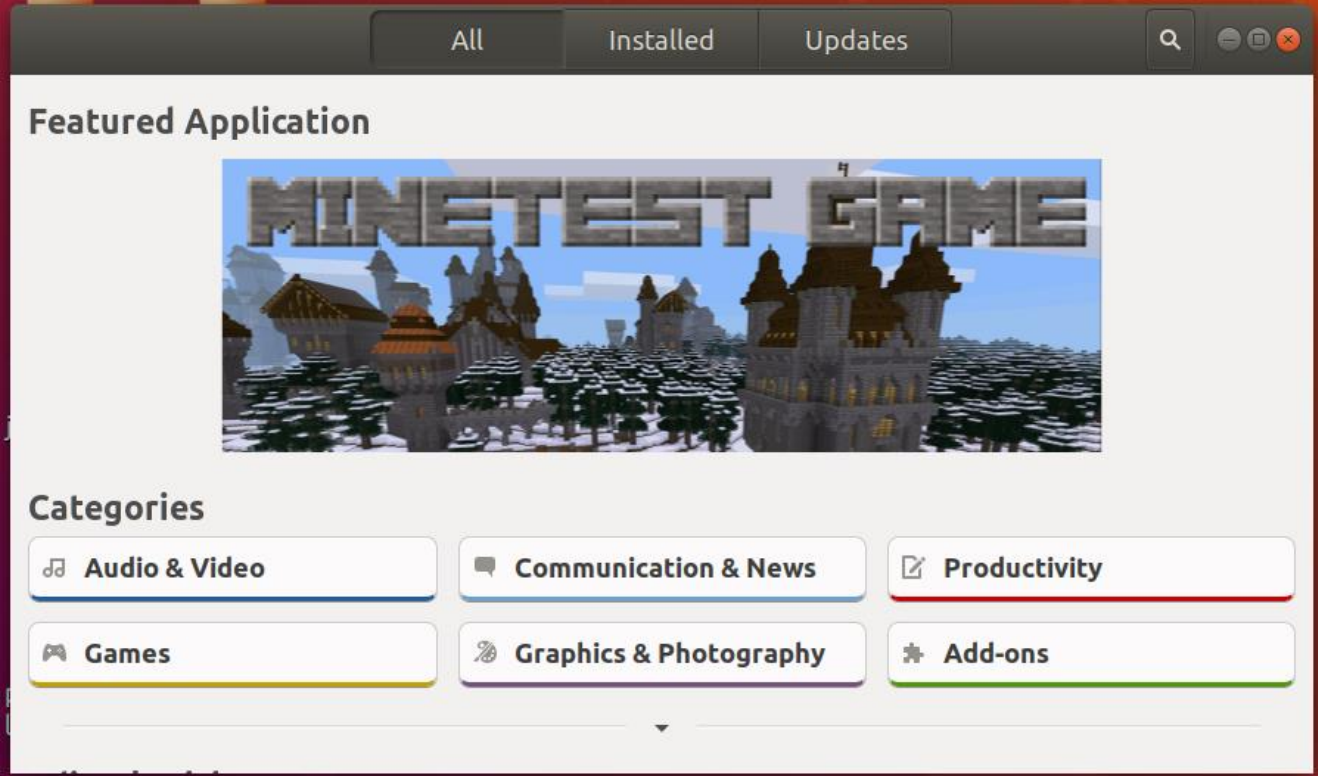
\includegraphics[width=\textwidth]{gnome.png}
            \caption{GNOME Software}
        \end{figure}
    \end{columns}
    
\end{frame}

\begin{frame}{软件安装}

    \begin{columns}
    
        \column{0.3\textwidth}
        
        应用商店
        
        搜索,

        点击安装,

        Done。
        
        \column{0.6\textwidth}
        \begin{figure}
            \centering
            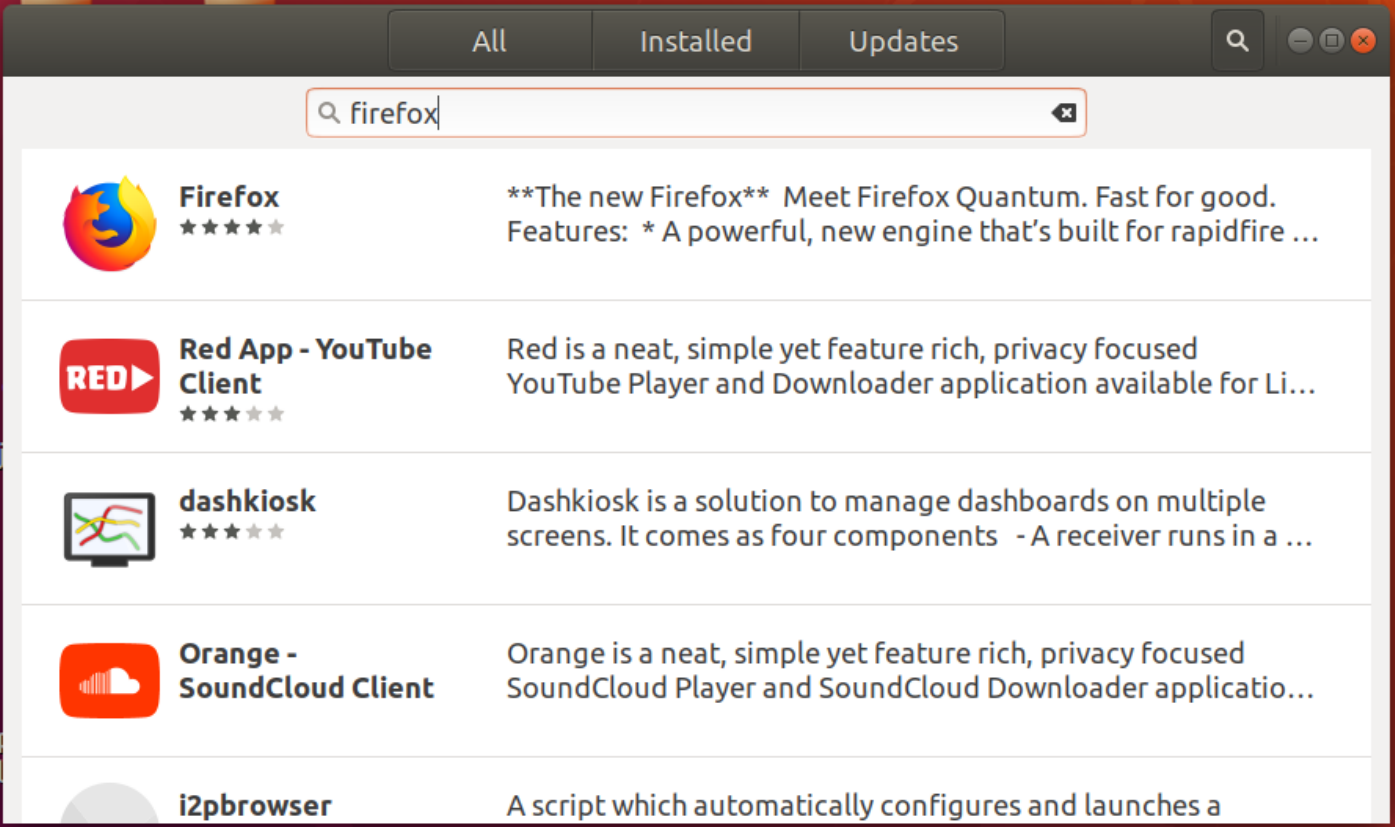
\includegraphics[width=\textwidth]{gnome-install.png}
            \caption{GNOME Software}
        \end{figure}
    \end{columns}
    
\end{frame}

\begin{frame}{软件安装}

    \begin{columns}
    
        \column{0.3\textwidth}
        
        应用商店
        
        Snap Store
        
        \href{https://snapcraft.io/store}{snapcraft.io}
        
        \column{0.6\textwidth}
        \begin{figure}
            \centering
            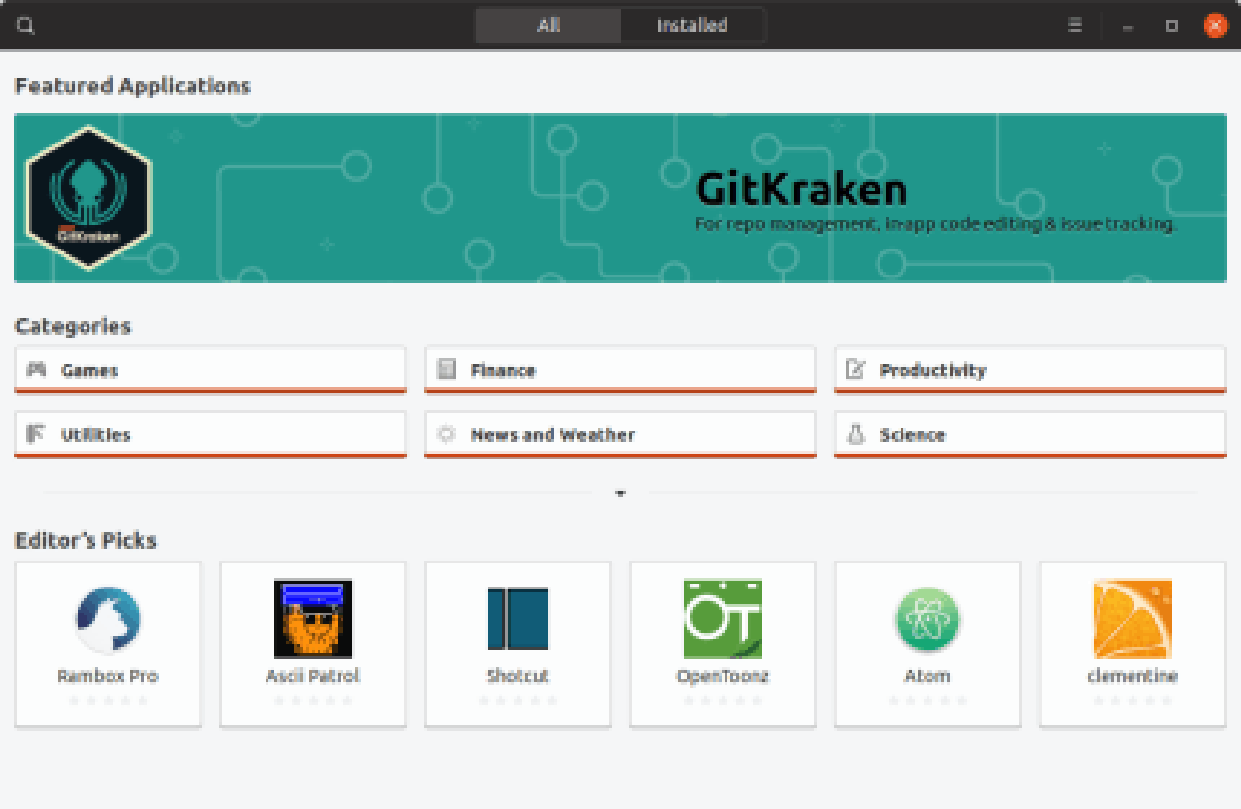
\includegraphics[width=\textwidth]{gnome-snap.png}
            \caption{Snap Store}
        \end{figure}
    \end{columns}
    
\end{frame}

\begin{frame}{软件安装}

    \begin{columns}
    
        \column{0.3\textwidth}
        
        应用商店
        
        上面的大多数为图形化的软件
        
        而 Linux 上面绝大多数都是命令行工具
        
        \column{0.6\textwidth}
        \begin{figure}
            \centering
            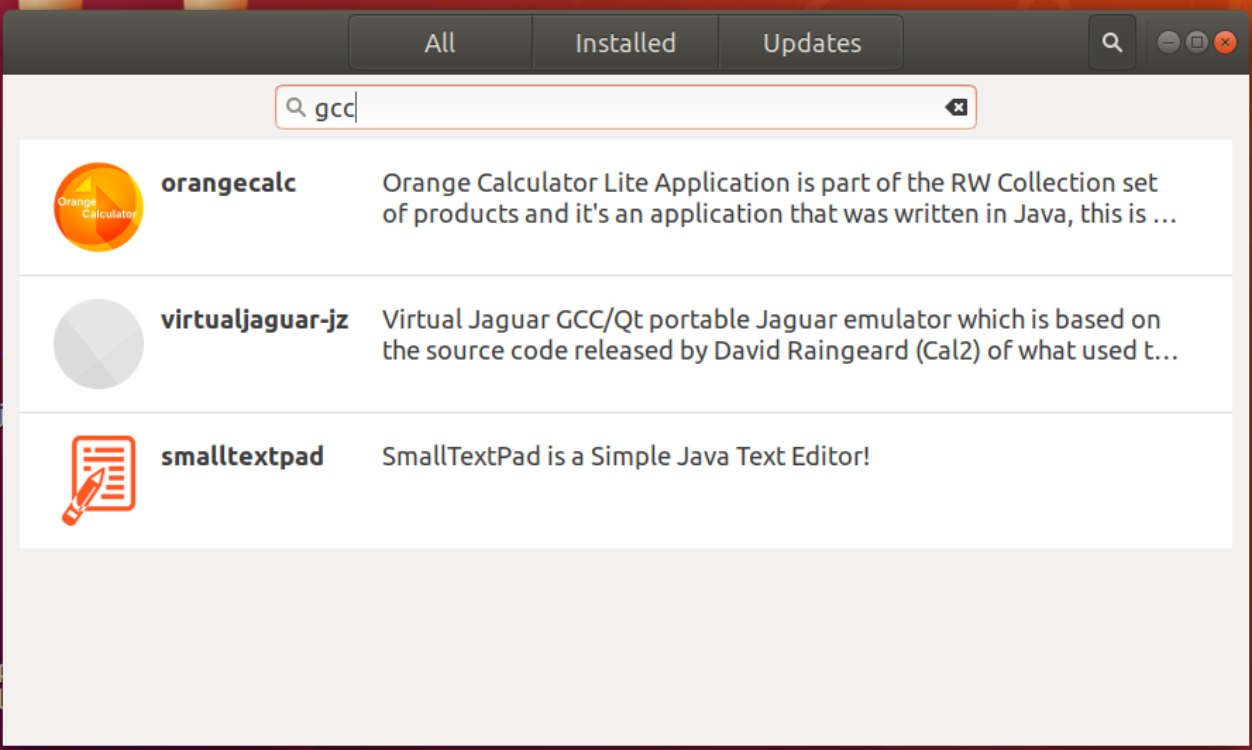
\includegraphics[width=\textwidth]{gnome-gcc.png}
            \caption{GNOME Software}
        \end{figure}
    \end{columns}
    
\end{frame}

\begin{frame}{软件安装}

    包管理器

    常见的包管理器前端:
    
    apt (Debian), yum (CentOS), pacman (Arch), apk (Apline) 等
    
    软件仓库是收藏了互联网上可用软件包的图书馆,包含成千上万的应用供用户安装。
    
    每个软件源中的软件列表便是丛书列表,软件包中也同时记录了软件所依赖的软件包。

\end{frame}

\begin{frame}{软件安装}

    包管理器
    
    使用 apt
    
    搜索:
    
    apt search + 软件名
    
    安装:
    
    apt install + 包名
    
    更新软件列表: apt update
    
    升级软件:
    
    apt upgrade
    
    例:clang和clang-9、clang-8、clang-7需要进行区分

\end{frame}

\begin{frame}{软件安装}

    包管理器
    
    软件安装速度慢?

    更换软件源!修改 /etc/apt/sources.list

    sudo sed -i 's/archive.ubuntu.com/mirrors.ustc.edu.cn/g' /etc/apt/sources.list

    切换完软件源后运行 apt update!

\end{frame}

\begin{frame}{软件安装}

    包管理器

    添加第三方软件源

    用于安装一些不在官方源中提供的软件,或者不同的版本

    例:docker-ce

    除了在 sources.list 内添加软件源条目以外,往往需要添加 GPG Key 以保证安全性

    deb [arch=amd64] https://download.docker.com/linux/ubuntu bionic stable

    \url{https://docs.docker.com/engine/install/ubuntu/\#install-using-the-repository}

\end{frame}

\begin{frame}{软件安装}


    包管理器手动安装

    一般用于安装 deb、rpm 这种文件

    并不会自动修复依赖关系

    dpkg –i <file>.deb

    修复依赖:

    apt -f install

    例:vscode

    \url{https://code.visualstudio.com/docs/setup/linux}

\end{frame}

\begin{frame}{软件安装}

    \begin{columns}
    
    \column{0.6\textwidth}

    预编译二进制文件

    需要软件提供商提前编译供用户下载

    即下即用,不需要安装

    可用于工具链多版本的管理

    安装指添加到 \$PATH 的路径下

    例:LLVM
    
    \column{0.35\textwidth}
    
    \begin{figure}
        \centering
        
\includegraphics[width=\textwidth]{llvm-logo.png}
        \caption{LLVM}
        \label{fig:llvm}
    \end{figure}
    
    \end{columns}

\end{frame}

\section{操作文件与文件夹}

\begin{frame}{操作文件与文件夹}

    创建一个空文件

    touch +文件名

    更新文件的时间戳

    : > a.txt

    true > a.txt

    echo -n > a.txt

    -n: do not output the trailing newline

    例:.gitkeep
    
\end{frame}

\begin{frame}{操作文件与文件夹}

    创建目录

    mkdir +目录

    同名文件与文件夹不能同时出现

    文件与文件夹的名称是区分大小写的

\end{frame}

\begin{frame}{操作文件与文件夹}

    拷贝、移动

    将 SOURCE 文件拷贝、移动到 DEST 文件,拷贝得到的文件即为 DEST

    cp/mv [OPTION] SOURCE DEST

    将 SOURCE 文件拷贝、移动到 DIRECTORY 目录下,SOURCE 可为多个文件

    cp/mv [OPTION] SOURCE... DIRECTORY

    常用的 [OPTION] :-r 递归复制、移动

\end{frame}

\begin{frame}{操作文件与文件夹}

    删除

    删除 FILE 文件,FILE 可以为多个文件

    rm [OPTION] FILE...

    常用的 [OPTION] :-r 递归删除,用于删除文件夹时

    删除文件夹:

    rmdir +目录(要求是空文件夹)

    rm -r +目录(不要求是空文件夹)

\end{frame}
\section{使用 tar 操作存档文件}

\begin{frame}{tar 操作存档}

    存档?

    存档是由多个文件加上一定的元数据组成的文件。

    常常用于将多个文件整合为一个文件,便于传输和存储、或者将文件进行压缩以便

    于减少存储空间的占用。

    创建 gzip 压缩的存档:

    一些文件 –> tar -> tar.gz

    Windows 上常见的存档为 .rar、.7z、.zip(带有压缩算法)
    
\end{frame}
\begin{frame}{tar 操作存档}

    创建存档

    tar -cf target.tar file…

    tar --create --file target.tar file…
    
\end{frame}
\begin{frame}{tar 操作存档}

    创建存档

    创建压缩的存档

    tar -czf target.tar.gz file…

    tar --create --gzip –file target.tar.gz file…

    常见的压缩算法由 gzip、bzip2、xz

    参数分别为 -z、-j、-J 或 --gzip、--bz、--xz
    
\end{frame}
\begin{frame}{tar 操作存档}

    追加文件到存档

    将 t2.tar 中的内容追加到 target.tar 存档中

    tar –Af target.tar t2.tar

    将 c 文件和 d 文件追加到 target.tar 存档中

    tar -rf target.tar c d

    tar --append --file target.tar c d
    
\end{frame}
\begin{frame}{tar 操作存档}

    查看存档的内容

    tar -t -f target.tar

    tar --list --file target.tar

    查看文件的详细信息

    tar -t -v -f target.tar

    tar --list --verbose --file target.tar
    
\end{frame}
\begin{frame}{tar 操作存档}

    从文档中提取文件

    tar -xf target.tar

    tar --extract --file target.tar

    提取到指定文件夹(文件夹要存在)

    tar -xf target.tar -C ./output\_folder

    解压特定的文件

    tar -xf target.tar -C ./output\_folder/ /path/to/file/relatively/in/archive

    所有没有跟在选项后的参数都需要放在最后

    tar 程序会识别文件头以选择合适的压缩算法
    
\end{frame}
\begin{frame}{tar 操作存档}

    unar 和 lsar
    
    apt install unar
    
    支持 zip 和 rar
    
    \url{https://theunarchiver.com/command-line}
    
\end{frame}
\section{软件的使用文档}
\begin{frame}{软件的使用文档}
    网络资源
    
    \url{http://man7.org/linux/man-pages/index.html}
    
    die.net
    
    Google Search: man tar
\end{frame}
\begin{frame}{软件的使用文档}

    man 命令
    
    软件安装时,会附带有使用文档,可以通过 man 命令获得
    
    得到的结果十分详细,大而全
    
    如:
    
    man ls
    
    man tar
    
\end{frame}

\begin{frame}{软件的使用文档}

    tldr 命令

    tldr = Too long; didn't read.

    可以快速了解一个程序的使用方法,而不用看大而全的官方使用文档

    tldr tar

    安装:

    apt install tldr
\end{frame}
\end{document}
